\documentclass[supercite]{Experimental_Report}

\title{LLM-DA：基于大语言模型的少样本命名实体识别数据增强方法\\\textit{LLM-DA: Data Augmentation via Large Language Models for Few-Shot Named Entity Recognition}}
\school{计算机科学与技术学院}
\author{瞿明睿}
\classnum{计科7班}
\stunum{U202215561}
\instructor{姚德中}

\usepackage{zhnumber}
\usepackage{amsmath}
\usepackage{amssymb}
\usepackage{amsfonts}
\usepackage{amsthm}
\usepackage[ruled,linesnumbered]{algorithm2e}
\usepackage{booktabs}
\usepackage{multirow}
\usepackage{graphicx}
\usepackage{subcaption}
\usepackage{framed}
\usepackage{mathtools}
\usepackage[table]{xcolor}
\usepackage{array}
\usepackage{float}
\usepackage{colortbl}
\usepackage{tabu}
\usepackage{xltxtra}
\usepackage{bm}
\usepackage{longtable}
\usepackage{tikz}
\usepackage{pdfpages}
\usepackage{tikzscale}
\usepackage{pgfplots}
\pgfplotsset{compat=1.16}

\usepackage[skins]{tcolorbox}
\tcbuselibrary{breakable}
\newtcolorbox{abox}[1][]{enhanced,
	fonttitle = \heiti \large \bfseries,
	colbacktitle =black,
	coltitle=white,
	attach boxed title to top left = {yshift = -5pt},
	fontupper = \kaishu,
	arc = 4pt,
	colframe=black,
	toprule  = 1pt,
	rightrule = 1pt,
	top = 10pt,
	title=#1,
	breakable
}

\newcommand{\cfig}[3]{
  \begin{figure}[htb]
    \centering
    \includegraphics[width=#2\textwidth]{images/#1}
    \caption{#3}
    \label{fig:#1}
  \end{figure}
}

\newcommand{\sfig}[3]{
  \begin{subfigure}[b]{#2\textwidth}
    \includegraphics[width=\textwidth]{images/#1}
    \caption{#3}
    \label{fig:#1}
  \end{subfigure}
}

\newcommand{\xfig}[3]{
  \begin{figure}[htb]
    \centering
    #3
    \caption{#2}
    \label{fig:#1}
  \end{figure}
}

\newcommand{\rfig}[1]{\autoref{fig:#1}}
\newcommand{\ralg}[1]{\autoref{alg:#1}}
\newcommand{\rthm}[1]{\autoref{thm:#1}}
\newcommand{\rlem}[1]{\autoref{lem:#1}}
\newcommand{\reqn}[1]{\autoref{eqn:#1}}
\newcommand{\rtbl}[1]{\autoref{tbl:#1}}

\newtheorem{thm}{定理}[section]
\newtheorem{lem}{引理}[section]
\renewcommand {\thefigure} {\arabic{figure}}
\colorlet{shadecolor}{black!15}

\theoremstyle{definition}
\newtheorem{alg}{算法}[section]
\def\thmautorefname~#1\null{定理~#1~\null}
\def\lemautorefname~#1\null{引理~#1~\null}
\def\algautorefname~#1\null{算法~#1~\null}

\newcommand{\tabincell}[2]{\begin{tabular}{@{}#1@{}}#2\end{tabular}}  

\begin{document}

\maketitle

\pagenumbering{Roman}
\pagenumbering{arabic}

\begin{abstract}
尽管大语言模型（LLMs）展现出令人印象深刻的能力，但它们在信息抽取任务上的表现仍然不尽如人意。然而，其卓越的文本重写能力和广泛的世界知识为改进这些任务提供了宝贵的思路。本文提出\emph{LLM-DA}，一种基于LLM的新型数据增强技术，用于少样本NER任务。为了克服现有数据增强方法损害语义完整性的局限，并解决LLM生成文本固有的不确定性问题，我们利用NER任务的独特特性，在上下文和实体两个层面增强原始数据。我们的方法包括采用14种上下文重写策略、设计同类型实体替换，并引入噪声注入以增强鲁棒性。大量实验证明了我们的方法在利用有限数据提升NER模型性能方面的有效性。此外，额外分析进一步证实了我们生成数据的质量优于其他现有方法。
\end{abstract}

\section{引言}
\label{sec:intro}

近年来，以ChatGPT为代表的一系列大语言模型（LLMs）引起了广泛关注\cite{instructGPT,PaLM,BLOOM,LLaMA,Llama-2}。这些模型使用来自各个领域的大量数据集进行训练，在各种自然语言处理（NLP）任务中展现出显著的竞争力\cite{transformers,GPT}。

\begin{figure}[!t]
    \centering
    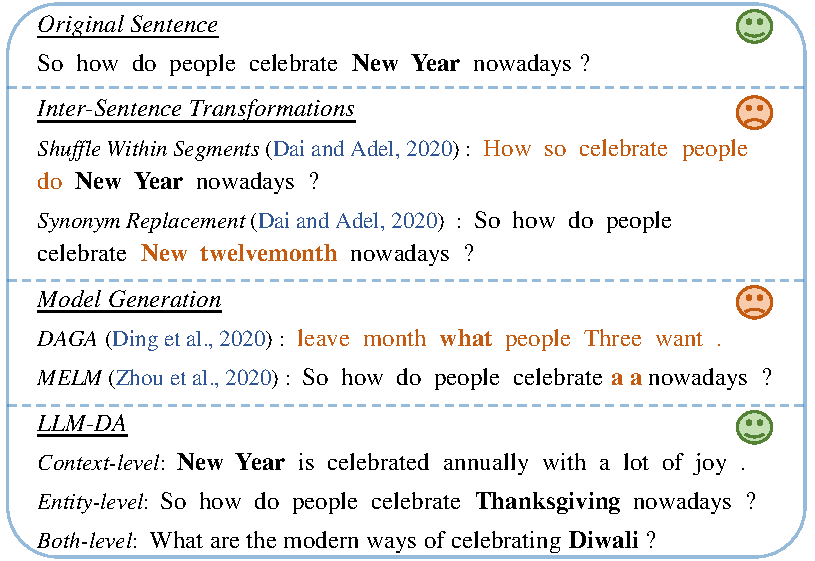
\includegraphics[width=\linewidth]{images/methods.pdf}
    \caption{应用于同一句原始句子的各种数据增强方法示例。句子中的实体（``event''）以\textbf{粗体}显示，任何不合语法或语义不连贯的部分以{\color[RGB]{197,90,17}红色}高亮标注。}
    \label{fig:augmented-data}
\end{figure}

大量研究表明，尽管GPT系列模型是目前可用的最强大的LLM，但它们在信息抽取任务上仍难以达到令人满意的性能\cite{InstructUIE,GPT-chen,GPT-ye,Stanford}。例如，GPT-3.5系列模型在命名实体识别（NER）任务上的micro-F1分数仅为20至60分。此外，针对特定领域训练专门的LLM也面临挑战，因为这需要大量的计算资源且应用受限。然而，LLM卓越的重写能力和庞大的世界知识为改进这些任务的处理提供了有前景的思路\cite{World-knowledge}。

考虑到NER训练数据中每个token标注的成本和挑战，标注样本的可用性有限\cite{huang2020few,fritzler2019few,SNN,template_based,template_free}。因此，我们主要关注解决训练数据稀缺场景下的NER问题。主流方法涉及使用数据增强技术生成额外的样本，这些方法可分为两类。第一类包括对给定句子应用变换操作，如实体替换、同义词替换和段落内混洗\cite{LSMS,EDA}。第二类涉及训练基础模型（如LSTM或RoBERTa），并利用其生成能力产生新数据\cite{DAGA,MELM,LSTM,RoBERTa}。

然而，现有方法往往会损害句子的语义完整性，如图~\ref{fig:augmented-data}所示。很明显，这些方法要么忽略了句子的句法结构（如段落内混洗和DAGA），要么忽略了上下文的语义（如同义词替换和MELM），阻碍了模型准确分析句子的能力。考虑到NER任务需要理解句子中每个token的句法结构和语义信息以准确识别实体及其对应类型，当前的数据增强技术可能会生成偏离事实准确性的句子，不利于有效的模型训练。

为解决这些问题，我们提出\emph{LLM-DA}，一种基于LLM的新型数据增强技术。LLM-DA利用LLM的文本生成能力产生符合实际表达惯例的语义连贯句子。然而，一个缺点在于LLM生成内容的高不确定性，这给处理生成数据带来了挑战。为了在保持增强数据多样性的同时对生成内容施加必要的约束，我们在上下文和实体两个层面应用数据增强。这种方法也符合NER任务的固有特性，其主要关注识别实体及其类别。

为了丰富\textbf{上下文层面的增强}，我们在四个维度提出了14种不同的上下文重写策略：句子长度、词汇使用、从句嵌入和呈现风格。这种扩展的策略组合旨在增强多样性同时保持语义连贯性。对于\textbf{实体层面的增强}，我们利用LLM广泛的世界知识将句子中的实体替换为同类型的其他实体。这使我们能够生成符合句子语义的多样化实体，超越训练数据的限制。为了进一步增强增强数据的多样性，我们采用\textbf{双层增强}方法，结合上述两种增强方法。此外，为了促进模型对输入变化的适应性，我们通过生成具有随机拼写错误的句子引入噪声注入。

我们将提出的方法四个变体的结果与其他四种基线方法进行比较。实验结果表明，我们的方法显著提升了模型在少样本NER任务上的性能。此外，通过对各种数据增强方法生成数据的综合分析，我们观察到LLM-DA始终如一地产生比其他方法更高质量的数据。

综上所述，本文的主要贡献如下：
\begin{itemize}
    \item 我们引入了一种利用LLM的世界知识和重写能力的新型数据增强方法。实验结果表明，我们的方法显著提升了NER任务的性能，特别是在训练样本有限的场景下。
    \item 我们在上下文和实体两个层面增强现有句子。为了确保生成数据的多样性和高质量，我们采用14种不同的上下文重写策略，并在数据增强过程中引入适当的噪声。
    \item 通过对生成数据的综合分析，我们展示了与现有方法相比，我们的方法在产生高质量句子方面始终具有优越性。此外，增强数据在多样性和可控性之间达到了和谐的平衡。
\end{itemize}

\begin{figure*}[!t]
    \centering
    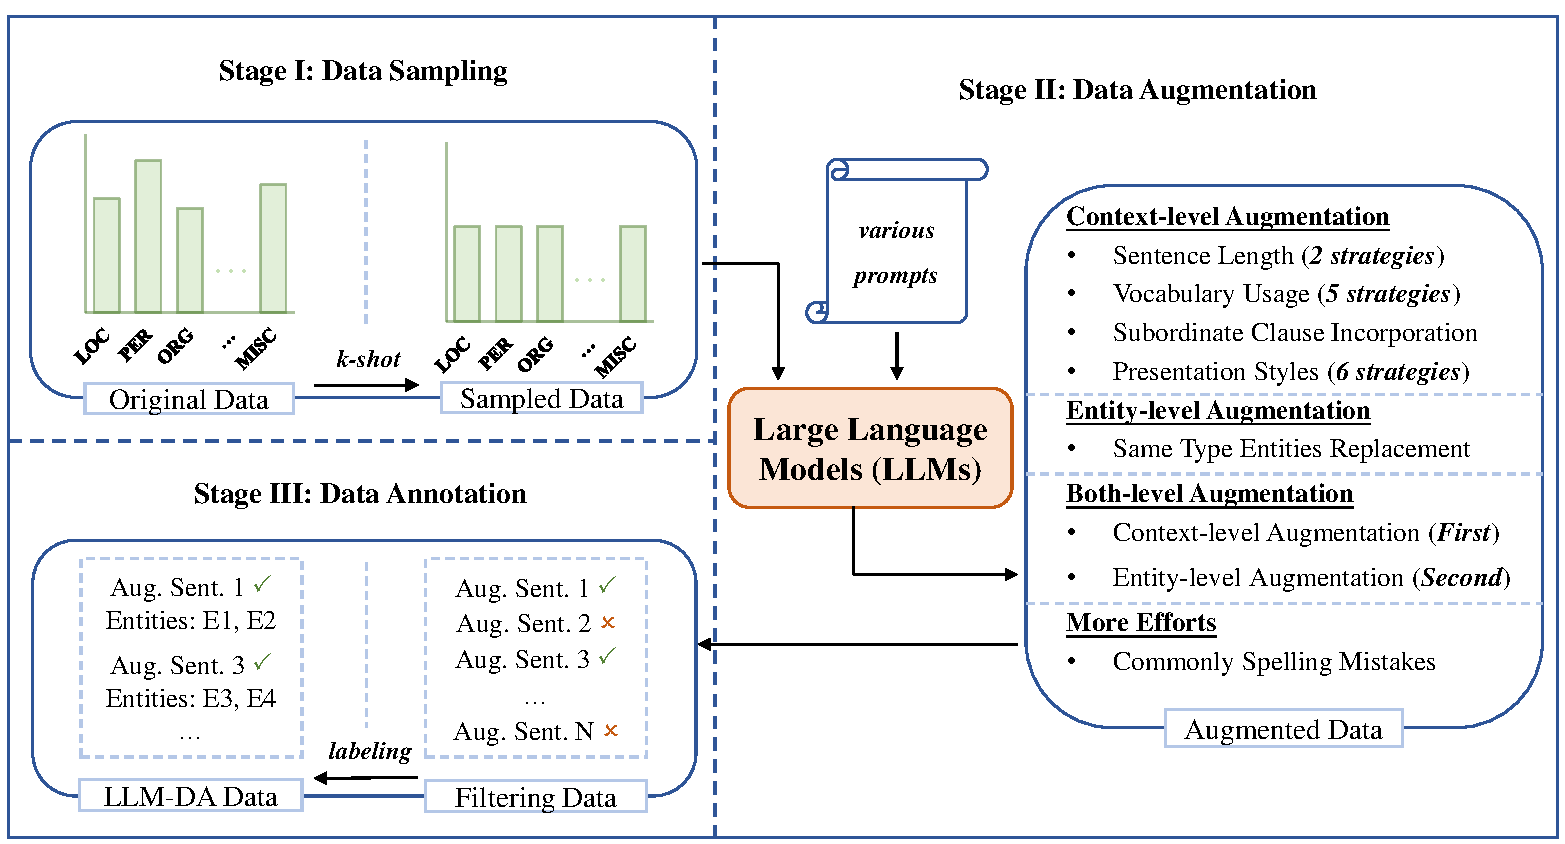
\includegraphics[width=\textwidth]{images/framework.pdf}
    \caption{LLM-DA示意图。LLM-DA包含三个阶段：从原始数据集进行数据采样、使用具有专门设计提示的LLM在四个维度生成增强数据，以及最后对增强数据进行过滤和标注以获得最终有效数据集。}
    \label{fig:LLM-DA}
\end{figure*}

\section{方法}

LLM-DA是一种主要依赖LLM的数据增强技术，利用其世界知识和重写能力扩展有限的标注数据，获取大量高质量数据。图~\ref{fig:LLM-DA}展示了LLM-DA的三个阶段：数据采样、数据增强和数据标注。以下章节将详细阐述这些阶段。

\subsection{数据采样}

\begin{algorithm}[!t]
    \caption{数据采样的贪心算法}
    \label{algorithm:sampling}
    \KwIn{shot数量$k$，带有标签集$\mathcal{Y}$的标注训练集$\mathrm{D}$。}
    \KwOut{采样得到的训练集$\mathrm{D_{smp}}$。}
    $\mathrm{D_{smp}} \gets \phi$ \tcp{初始化采样训练集。}
    
    \For{$\forall y \in \mathcal{Y}$}{
    {Count}$[y]$ $\gets 0$
    }

    $\mathrm{Shuffle~D}$

    \For{$(X,Y) \in \mathrm{D}$}{
    $add \gets \mathrm{True}$

        \For{$y \in \mathcal{Y}$}{
        $\mathrm{Count_{tmp}}[y] \gets$ $(X,Y)$中$y$的提及数量

        \If{$\mathrm{Count}[y]+\mathrm{Count_{tmp}}[y]>1.25 \times k$}{$add \gets \mathrm{False}$}
        }

        \If{$add==\mathrm{True}$}{
        $\mathrm{D_{smp}} \gets \mathrm{D_{smp}} \cup (X,Y)$

        \For{$y \in \mathcal{Y}$}{
        $\mathrm{Count}[y] \gets \mathrm{Count}[y] + \mathrm{Count_{tmp}}[y]$
        }
        }
        \If{$\forall$ $y \in \mathcal{Y}$, $\mathrm{Count}[y]>=k$}{$\mathrm{break}$ \tcp{完成采样。}}
    }
\end{algorithm}

给定标注训练集$\mathrm{D}=\{(X_i, Y_i)\}_{i=1}^{\vert \mathrm{D} \vert}$，其中$\vert \mathrm{D} \vert$表示$\mathrm{D}$中的样本数量，我们的方法涉及使用贪心算法（算法~\ref{algorithm:sampling}）采样$k$-shot示例。在NER任务的背景下，标准$k$-shot样本指在样本中为每个类别获取恰好$k$个实体出现。然而，满足这一严格要求可能具有挑战性，特别是处理标签分布不平衡的数据时。为解决这一挑战，我们借鉴FEW-NERD的工作\cite{Few-NERD}，引入对标准的放宽。这种放宽允许在$k$-shot场景中每个类别最多出现$1.25k$个实体。我们的方法考虑了现实世界中实体类别分布的固有偏倚，同时尽可能保持$k$-shot设置。这种方法能够更好地捕捉真实世界数据的分布。

\subsection{数据增强}

由于LLM不需要使用数据进行参数微调，精心设计适当的提示对于充分利用其能力至关重要。借鉴已建立的原则性指导和考虑到NER任务涉及在给定句子中识别实体及其类型的独特性质，我们为上下文和实体两个层面的数据增强构建了专门的提示。

\paragraph{上下文层面增强}
MELM的前期工作表明，简单的上下文替换带来的改进有限。为了使文本多样化，我们在四个不同维度整合了重写方法，借鉴了先前的语言学研究。我们的目标是为给定输入句子及其相关实体生成14种句子变体。这些变体涵盖了句子长度（即长句和短句）、词汇使用（即高级词汇、副词、形容词、介词和连词）、从句嵌入和呈现风格（即新闻、口语、杂志、小说、维基百科和电影评论）等不同方面。在此过程中，我们获得了一组重写上下文的新句子，同时保留了原始句子中的实体。

\paragraph{实体层面增强}
我们指示模型将给定句子中的实体替换为同类型的其他实体，同时保持原始句子结构。与现有的实体替换方法不同，我们的方法利用嵌入在LLM中的世界知识，允许生成训练集中不存在的实体。此外，为了增强数据多样性，我们在遵守模型token长度限制的前提下尽可能多地生成句子。这种策略大大扩展了实体的范围，并为增强数据的整体丰富性做出了贡献。

\paragraph{双层增强}
在上下文和实体层面增强的基础上，我们自然地将这两种方法结合在给定句子中。然而，当两个层面同时重写时，生成内容的固有不确定性往往导致新句子与原始句子显著偏离，给标签处理带来挑战。为解决这一问题，我们采用两阶段策略：首先执行上下文层面增强，然后基于已生成的上下文增强句子进行实体层面增强。通过采用这种策略，我们在保持新生成句子与原始句子之间有意义的关联的同时，实现了有效的数据多样化。

此外，为了提高下游模型的鲁棒性，我们指示LLM用常见的拼写错误随机替换原始句子中的某些词。为了确保模型从引入的噪声中获益而不受过度影响，我们为每个原始句子最多生成一个带有噪声的增强句子。

\subsection{数据标注}

虽然我们已在提示中引入各种约束来指导LLM的输出，但重要的是要承认生成模型可能仍然会产生与我们的要求不一致的内容。为克服这一问题，我们对生成数据实施了一个简单的过滤过程。具体而言，对于上下文层面增强的数据，我们丢弃模型保留除给定实体之外其他实体的句子。类似地，对于其他类型的增强数据，我们移除模型修改非给定实体的句子。对于过滤后的句子，我们分配与原始句子相同的标签。这意味着保留或替换的实体被标记为其原始实体类型，而剩余的token被标记为非实体类型。

\section{实验设置}

\subsection{任务定义}

我们主要通过将我们的方法与现有方法在少样本NER任务上的性能进行比较来评估我们的方法。在NER任务中，给定候选实体标签$\mathrm{E}$和token序列$x = (x_1, x_2, ..., x_n)$。模型的目标是预测实体标签$y = (y_1, y_2, ... y_n)$，其中每个$y_i \in \mathrm{E}$对应于$x$中的一个token。$k$-shot NER任务指训练集中每个实体大约出现$k$次的场景，这可能无法为模型提供足够的训练数据。

\begin{table}[!t]
    \centering
    \resizebox{\linewidth}{!}{%
    \begin{tabular}{lcccccc}
    \toprule
    {数据集} & {类别数} & {5-shot} & {10-shot} & {15-shot} & {20-shot} & {测试集} \\
    \midrule
    CoNLL'03 & 4 & 10 & 20 & 30 & 40 & 3.7k \\
    OntoNotes 5.0 & 11 & 50 & 100 & 140 & 190 & 8.3k \\
    MIT Movie & 12 & 45 & 90 & 135 & 180 & 2.4k \\
    FEW-NERD & 66 & 250 & 435 & 620 & 860 & 37.6k \\
    \bottomrule
    \end{tabular}
    }
    \caption{数据集统计信息。``$k$-shot''列表示该场景中采样的数据数量。}
    \label{datasets}
\end{table}

\subsection{数据集}

我们使用四个涵盖不同领域且具有不同粒度级别的NER数据集全面评估我们的方法。这些数据集包括新闻领域的CoNLL'03、通用领域的OntoNotes 5.0、评论领域的MIT-Movie以及通用领域的FEW-NERD。关于每个数据集的详细信息见表~\ref{datasets}。

\subsection{基线方法}

\paragraph{数据增强方法}
为评估我们方法的有效性，我们在实验中将其与四种基线方法进行比较：1）\textbf{Gold}使用原始采样数据作为训练样本训练NER模型；2）\textbf{LSMS}利用四种句子变换生成增强数据，包括标签级token替换、同义词替换、提及替换和段落内混洗；3）\textbf{DAGA}使用带有线性化标签的序列训练LSTM模型，并利用该模型生成用于训练的新数据；4）\textbf{MELM}训练RoBERTa模型，通过替换序列中的实体来生成增强数据。同时，我们将我们的方法分为四个不同的类别：1）\textbf{LLM-DA (Context)}使用上下文层面增强数据作为训练数据；2）\textbf{LLM-DA (Entity)}使用实体层面增强数据以及噪声注入数据作为训练数据；3）\textbf{LLM-DA (Both)}将双层增强数据作为训练数据；4）\textbf{LLM-DA (All)}将LLM-DA (Context)、LLM-DA (Entity)和LLM-DA (Both)的数据合并用于训练。

\paragraph{分类模型}
为对我们提出的方法与现有数据增强方法在少样本NER任务上的性能进行全面比较，我们使用两种已建立的预训练掩码语言模型，随后对其进行微调用于评估：1）\textbf{BERT}是一种基于Transformer编码器架构的大规模预训练模型，广泛用于各种NLP任务；2）\textbf{RoBERTa}是BERT的改进版本，是该领域最先进的预训练分类模型之一。

\begin{table}[!t]
    \centering
    \resizebox{\linewidth}{!}{
    \begin{tabular}{lcccc}
    \toprule
         方法 & CoNLL'03 & OntoNotes 5.0 & MIT-Movie & FEW-NERD \\ \midrule
         LLM-DA (Context) & 45$\times$ & 20$\times$ & 30$\times$ & 10$\times$ \\
         LLM-DA (Entity) & 20$\times$ & 18$\times$ & 20$\times$ & 15$\times$ \\
         LLM-DA (Both) & 40$\times$ & 12$\times$ & 25$\times$ & 7$\times$ \\
         LLM-DA (All) & 105$\times$ & 50$\times$ & 75$\times$ & 30$\times$ \\ \bottomrule
    \end{tabular}}
    \caption{不同方法在不同数据集上相对于``Gold''条目的增强率。}
    \label{table:aug-rate}
\end{table}

\subsection{实验设置细节}

我们的实验包含两个阶段：数据增强和模型验证。

在数据增强阶段，我们使用OpenAI开发的gpt-3.5-turbo，这是GPT-3.5子系列中最强大的模型\cite{instructGPT,GPT}。为充分发挥其能力，我们将模型的最大输出长度设置为2048个token。为保证实验结果的可复现性，我们通常将温度参数设置为0。然而，在双层数据增强阶段，我们将温度参数设置为1以增强实体的多样性。

需要注意的是，由于不同数据集的标签数量和样本大小不同，我们的增强倍数也有所差异。具体的增强倍数数值见表~\ref{table:aug-rate}。在涉及相同数据集的情况下，除了某些基线方法（如MELM）在原始论文中指定了最佳增强率外，我们将其他方法的增强率调整为与LLM-DA (All)的增强率相匹配。这种仔细的调整确保了实验结果的公平比较。

在模型验证阶段，我们使用inside-outside标注方案将增强数据与原始数据合并。在实验中，我们将batch size设置为8，使用AdamW优化器，学习率为3e-5。模型训练20个epoch，选择在验证集上表现最好的模型进行测试。同时，我们实施早停策略，如果5个epoch内没有改进则终止训练。

此外，为减轻标注过程中产生的标签噪声的影响，我们对我们方法和所有数据增强基线使用广义交叉熵损失\cite{GCELoss}：
\begin{equation*}
    \mathrm{GCELoss}_q(\hat{y}, e_j)=\frac{1-\hat{y}_j^q}{q}
\end{equation*}
其中$\hat{y}$表示预测的概率分布，$e_j$表示实际标签为类别$j$，$\hat{y_j}$表示预测为类别$j$的概率，$q$是统一设置为0.5的超参数。对于基线``Gold''，我们假设其无噪声并使用交叉熵损失。

\section{实验分析}

\subsection{主要结果}

我们通过将我们的方法与现有方法在四个少样本设置（5-shot、10-shot、15-shot和20-shot）上进行比较来评估我们的方法。我们进行10次独立重复实验，计算每种方法的micro-F1分数的均值和标准差。结果总结在表~\ref{tab:main_result}中。从实验结果中，我们有以下观察。

\begin{table*}[!t]
    \centering
    \resizebox{\textwidth}{!}{
        \begin{tabular}{l|l|cccc|cccc}
        \toprule
        \multirow{2}*{数据集} &  \multirow{2}*{方法} & \multicolumn{4}{c|}{{BERT-base-cased}} & \multicolumn{4}{c}{{RoBERTa-base}} \\
       ~ & ~ & 5-shot & 10-shot & 15-shot & 20-shot & 5-shot & 10-shot & 15-shot & 20-shot \\
       \midrule
       
        \multirow{9}*{{CoNLL'03}} & Gold & 1.58 (0.16) & 3.33 (6.44) & 8.72 (16.13) & 34.39 (23.60) & 3.95 (1.06) & 3.35 (0.79) & 3.45 (0.26) & 33.90 (20.36) \\
        ~ & LSMS & 34.25 (7.80) & 50.06 (3.02) & 57.76 (4.06) & 61.28 (2.73) & 31.14 (11.08) & 47.83 (2.94) & 52.30 (3.99) & 56.94 (3.10) \\ 
        ~ & DAGA & 17.11 (9.37) & 40.22 (7.79) & 39.51 (14.24) & 46.26 (4.82) & 3.04 (4.97) & 8.89 (12.54) & 2.98 (3.39) & 13.45 (11.70) \\
        ~ & MELM & 1.05 (2.16) & 7.59 (12.13) & 35.49 (4.58) & 45.71 (3.41) & 4.35 (0.97) & 1.69 (2.21) & 38.29 (7.36) & 39.99 (5.78) \\
        \rowcolor{gray!10} \cellcolor{gray!0}CoNLL'03 & \cellcolor{gray!10}LLM-DA (Context) & \underline{40.51 (7.46)} & 51.79 (4.74) & 58.87 (4.19) & 62.74 (3.79) & \underline{44.50 (8.39)} & \underline{50.82 (2.20)} & \underline{55.54 (2.83)} & 57.77 (2.72) \\
        \rowcolor{gray!10} \cellcolor{gray!0}~ & LLM-DA (Entity) & \underline{39.53 (9.02)} & \underline{51.48 (3.73)} & 57.57 (3.41) & 62.92 (2.26) & \underline{36.25 (9.59)} & 48.72 (3.70) & \underline{55.49 (3.95)} & 57.92 (3.23) \\
        \rowcolor{gray!10} \cellcolor{gray!0}~ & LLM-DA (Both) & \underline{52.78 (5.99)} & \underline{60.22 (3.05)} & \underline{65.68 (3.52)} & \underline{66.21 (3.25)} & \underline{52.56 (5.38)} & \underline{58.10 (2.93)} & \underline{61.39 (3.81)} & \underline{63.96 (2.80)} \\ 
        \rowcolor{gray!10} \cellcolor{gray!0}~ & LLM-DA (All) & \underline{\textbf{54.04} (5.93)} & \underline{\textbf{61.25} (3.08)} & \underline{\textbf{66.64} (2.70)} & \underline{\textbf{67.68} (2.47)} & \underline{\textbf{54.62} (4.14)} & \underline{\textbf{59.32} (3.56)} & \underline{\textbf{64.05} (1.78)} & \underline{\textbf{64.40} (2.22)} \\
        \midrule
        
        \multirow{9}*{{OntoNotes 5.0}} & Gold & 10.34 (7.68) & 38.41 (4.48) & 49.44 (1.52) & 57.56 (3.19) & 0.08 (0.01) & 18.57 (7.89) & 35.12 (10.12) & 49.65 (5.08) \\ 
        ~ & LSMS & 39.90 (3.64) & 53.19 (3.09) & 58.47 (1.64) & \textbf{64.02} (2.66) & 36.96 (6.58) & 47.74 (3.76) & 52.71 (2.82) & \textbf{59.75} (1.45) \\ 
        ~ & DAGA & 6.42 (4.54) & 17.26 (14.19) & 24.62 (18.71) & 19.84 (20.67) & 0.01 (0.04) & 0.16 (0.35) & 6.90 (12.39) & 4.69 (8.72) \\
        ~ & MELM & 0.54 (1.04) & 36.17 (2.75) & 48.25 (3.32) & 55.42 (2.22) & 5.96 (6.60) & 23.11 (8.22) & 38.87 (5.11) & 44.26 (14.91) \\ 
        \rowcolor{gray!10} \cellcolor{gray!0}OntoNotes 5.0 & LLM-DA (Context) & {34.54 (6.01)} & {46.75 (4.39)} & {52.12 (2.91)} & 57.34 (3.24) & {28.07 (4.52)} & {37.84 (4.98)} & {45.02 (4.21)} & 50.90 (3.27) \\ 
        \rowcolor{gray!10} \cellcolor{gray!0}~ & LLM-DA (Entity) & 42.68 (5.32) & \textbf{54.79} (2.89) & \textbf{58.52} (3.34) & 63.62 (1.94) & {27.08 (9.53)} & 45.66 (5.98) & \textbf{54.27} (4.58) & {57.77 (2.54)} \\ 
        \rowcolor{gray!10} \cellcolor{gray!0}~ & LLM-DA (Both) & \underline{44.25 (6.75)} & {50.66 (3.72)} & {52.80 (2.52)} & 55.54 (2.58) & 40.01 (5.49) & 46.12 (3.90) & {49.65 (4.34)} & {54.26 (3.02)} \\ 
        \rowcolor{gray!10} \cellcolor{gray!0}~ & LLM-DA (All) & \underline{\textbf{46.35} (5.01)} & 51.89 (2.99) & {55.74 (3.11)} & {60.05 (2.27)} & \underline{\textbf{43.92} (5.68)} & \underline{\textbf{50.29} (4.01)} & 53.97 (2.74) & {56.97 (2.24)} \\
        \midrule
        
        \multirow{9}*{{MIT-Movie}} & Gold & 17.59 (9.38) & 49.17 (2.57) & 55.89 (2.84) & 61.94 (2.06) & 2.88 (6.16) & 49.30 (2.45) & 57.23 (2.58) & 64.50 (1.41) \\
        ~ & LSMS & 45.28 (2.34) & 56.64 (2.43) & 60.01 (2.38) & 65.80 (1.46) & 46.84 (2.87) & 59.78 (2.53) & 63.09 (2.02) & 66.69 (1.46) \\
        ~ & DAGA & 27.68 (5.89) & 39.89 (4.93) & 38.99 (4.17) & 47.61 (3.56) & 3.37 (5.54) & 11.35 (7.16) & 23.75 (9.20) & 44.17 (6.06) \\ 
        ~ & MELM & 37.08 (4.37) & 54.39 (1.76) & 59.57 (1.82) & 64.71 (1.58) & 30.54 (2.68) & 51.87 (2.87) & 58.09 (1.79) & 63.17 (1.43) \\
        \rowcolor{gray!10} \cellcolor{gray!0}MIT-Movie & LLM-DA (Context) & {42.67 (4.05)} & 54.93 (1.95) & 56.62 (2.10) & 61.72 (2.43) & {39.05 (2.28)} & 52.32 (2.66) & {55.41 (1.91)} & {60.23 (2.96)} \\ 
        \rowcolor{gray!10} \cellcolor{gray!0}~ & LLM-DA (Entity) & \underline{49.20 (4.16)} & \underline{62.32 (2.15)} & \underline{63.96 (2.14)} & \underline{\textbf{68.71} (1.01)} & \underline{55.76 (5.21)} & \underline{\textbf{66.86} (1.56)} & \underline{67.13 (1.29)} & \underline{\textbf{70.49} (1.11)} \\ 
        \rowcolor{gray!10} \cellcolor{gray!0}~ & LLM-DA (Both) & \underline{51.08 (4.82)} & \underline{59.61 (1.37)} & 60.87 (2.78) & 66.18 (1.58) & \underline{54.23 (5.57)} & \underline{62.67 (1.90)} & 64.02 (1.54) & 66.85 (1.71) \\ 
        \rowcolor{gray!10} \cellcolor{gray!0}~ & LLM-DA (All) & \underline{\textbf{52.85} (3.70)} & \underline{\textbf{62.80} (1.22)} & \underline{\textbf{64.86} (2.21)} & \underline{68.55 (1.69)} & \underline{\textbf{58.94} (3.99)} & \underline{66.07 (2.01)} & \underline{\textbf{67.65} (1.98)} & \underline{70.24 (1.21)} \\
        \midrule
        
        \multirow{9}*{{FEW-NERD}} & Gold & 18.82 (1.28) & 32.23 (1.95) & 39.29 (1.79) & 43.47 (0.80) & 12.45 (1.86) & 29.47 (1.51) & \textbf{38.76} (1.93) & \textbf{43.03} (1.35) \\ 
        ~ & LSMS & 28.00 (2.56) & 35.53 (1.67) & 39.72 (1.84) & 42.71 (1.08) & 24.19 (2.98) & 32.27 (1.72) & 36.59 (2.30) & 40.94 (1.62) \\ 
        ~ & DAGA & 0.15 (0.48) & 20.38 (5.60) & 30.05 (10.82) & 38.01 (8.41) & 0.13 (0.31) & 11.13 (9.16) & 22.59 (12.39) & 30.11 (14.19) \\ 
        ~ & MELM & 22.42 (4.10) & 35.11 (3.50) & 40.71 (1.79) & \textbf{44.36} (2.14) & 19.42 (2.57) & 33.42 (2.30) & 38.66 (2.69) & 41.70 (1.33) \\ 
        \rowcolor{gray!10} \cellcolor{gray!0}FEW-NERD & LLM-DA (Context) & 23.60 (1.81) & {30.02 (2.24)} & 34.56 (1.72) & 37.81 (1.78) & 17.76 (2.34) & {26.00 (2.62)} & {32.74 (1.91)} & 35.66 (1.79) \\ 
        \rowcolor{gray!10} \cellcolor{gray!0}~ & LLM-DA (Entity) & \underline{\textbf{33.98} (2.80)} & \underline{\textbf{39.87} (1.29)} & \textbf{41.67} (2.26) & 43.88 (1.72) & \underline{\textbf{31.89} (1.83)} & \underline{\textbf{36.40} (1.90)} & 37.84 (2.48) & 40.20 (1.50) \\ 
        \rowcolor{gray!10} \cellcolor{gray!0}~ & LLM-DA (Both) & \underline{32.35 (1.45)} & 36.64 (1.68) & 39.35 (1.44) & 41.05 (1.21) & \underline{29.65 (1.62)} & 34.15 (2.42) & 37.44 (1.81) & {39.61 (1.11)} \\ 
        \rowcolor{gray!10} \cellcolor{gray!0}~ & LLM-DA (All) & \underline{32.02 (1.43)} & 36.42 (1.30) & 38.97 (2.67) & 40.42 (1.61) & \underline{29.55 (1.53)} & \underline{34.86 (1.11)} & 36.43 (1.59) & {38.61 (1.95)} \\
        \bottomrule
        
        \end{tabular}}
    \caption{基于micro-F1分数的评估结果。``$k$-shot''（$k \in \{5, 10, 15, 20\}$）指每种标签类型出现$k$次。我们使用不同的随机种子对所有实验进行十次独立重复。报告均值和标准差。每种设置中的最佳结果以\textbf{粗体}突出显示。\underline{下划线}结果表示通过配对Student's t检验（p值小于0.05）显著优于所有基线方法。}
    \label{tab:main_result}
\end{table*}

\paragraph{性能提升}
在资源有限的场景中，与现有方法相比，我们的方法始终能够提升模型性能。例如，在仅包含四种实体类型的CoNLL'03数据集\cite{IO-scheme}上，与任何其他现有方法相比，我们的方法展现出至少30分的显著性能提升。同样，在包含66种细粒度实体类型的FEW-NERD数据集\cite{Few-NERD}上，在5/10-shot设置中，我们的方法比无数据增强方法高出5-15分。

\paragraph{策略比较}
通过综合表~\ref{datasets}和表~\ref{tab:main_result}的见解，我们可以辨别不同层面数据增强方法对各种数据集模型性能的影响。一个有趣的观察浮现：当处理较小的数据集（如CoNLL'03数据集）时，与仅依赖实体层面增强相比，双层和上下文层面增强产生更明显的性能改进。这一观察凸显了所考察的14个领域中上下文层面增强策略在提升模型性能方面的有效性。此外，双层增强充分利用了上下文层面和实体层面增强的优势，在特定场景下提供了最佳结果。

然而，随着数据集规模的增加，上下文层面增强的优势逐渐减弱，而实体层面增强的好处持续增长，可能超过双层增强。我们推测这种性能动态的转变可以归因于模型对拟合实体信息而非上下文信息的关注日益增加。此外，上下文层面增强将测试集中的变化引入增强数据分布，这在更大的数据集中变得更加明显，最终对性能产生负面影响。这一缺点也延伸到双层增强，它依赖上下文层面增强数据作为进一步变化的基础，加剧了对性能的负面影响。

\begin{figure}[!t]
    \centering
    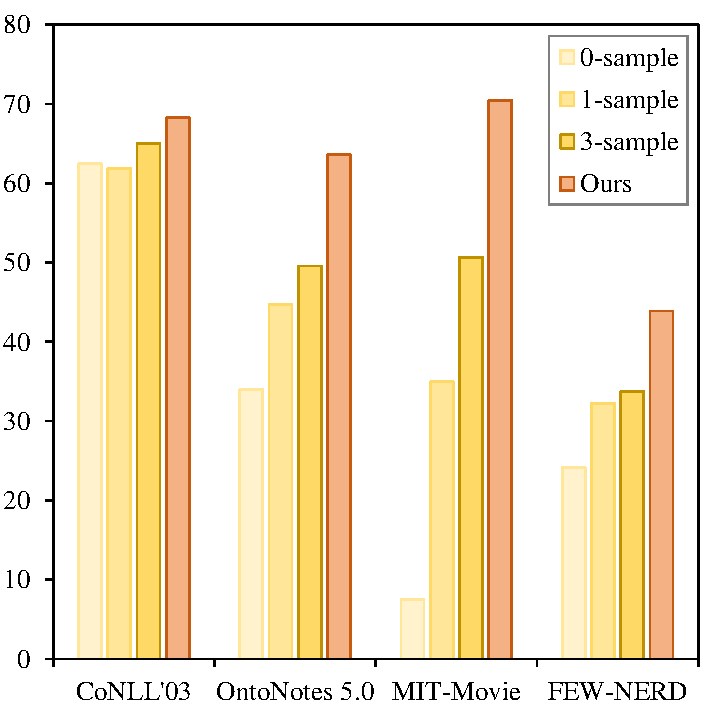
\includegraphics[width=0.8\linewidth, height=0.5\linewidth]{images/gpt_test.pdf}
    \caption{使用0/1/3个样本的ChatGPT性能与使用LLM-DA数据训练的较小模型的对比。}
    \label{fig:performace-gpt}
\end{figure}

\paragraph{适用场景}
与替代方法相比，LLM-DA在两种场景下提供更明显的优势。一方面，它在\textbf{极端低资源场景}中表现出色。在5-shot场景中，LLM-DA在所有四个数据集上比其他方法获得了显著更大的性能提升。然而，需要注意的是，随着示例数量的增加，这种好处会逐渐减弱。特别是在处理FEW-NERD数据集时，在包含约860个数据样本的20-shot设置中，使用任何数据增强方法都可能对模型性能产生负面影响。尽管如此，与其他方法相比，LLM-DA仍然保持较高的整体性能。这是因为在超过一定数据量阈值后，数据增强引入的噪声的不利影响可能超过增加数据带来的优势。

另一方面，当处理\textbf{领域特定数据}时，LLM-DA证明非常有效。在与我们的上下文层面增强领域一致的数据集（如CoNLL'03和MIT-Movie）上，我们方法的大多数结果显著优于所有其他方法。然而，在OntoNotes 5.0和FEW-NERD等数据集上，虽然我们的方法总体上优于其他方法，但少数方法设法取得了可比较的结果。这种差异可能源于我们的方法对增强数据施加了某些约束，而没有自动适应数据对应的特定领域。

\subsection{ChatGPT性能分析}

为直接评估LLM在NER任务上的性能，我们采用ChatGPT作为代表在四个数据集上进行评估。遵循先前研究评估ChatGPT在NER任务上性能的实验协议，我们在零样本和少样本场景下进行测试。然而，由于ChatGPT的\emph{token长度限制}，我们最多只能同时纳入三个示例。我们最终评估的结果如图~\ref{fig:performace-gpt}所示。

对结果进行全面分析后，出现了几个关键观察：1）我们的方法在所有四个数据集上始终优于ChatGPT在NER任务上的表现。当我们使用LLM-DA增强数据时，较小的模型始终超越ChatGPT。值得注意的是，ChatGPT仅在CoNLL'03数据集的情况下显示出与我们的方法接近的结果，该数据集仅包含四个标签。这种观察可以归因于数据集的简单性及其作为广泛使用的公共基准的地位，这引发了ChatGPT可能在训练期间遇到过它的可能性。因此，我们方法的实际效益将变得更加明显；2）ChatGPT不适合直接应用于NER任务，这与GPT-ye的发现一致\cite{GPT-ye,Stanford}。这种局限性在解决具有更多标记类型多样性的数据集（如MIT-Movie和FEW-NERD）时尤为明显；3）与in-context一致\cite{in-context}，示例未能缓解ChatGPT在NER任务上的性能挑战。ChatGPT的上下文约束阻碍了我们引入额外示例的能力，并且这种添加带来的性能增益似乎随时间推移而减弱。

\subsection{语言质量分析}

\begin{table}[!t]
    \centering
    \resizebox{\linewidth}{!}{%
    \begin{tabular}{lcccc}
    \toprule
    {方法} & LSMS & DAGA & MELM & LLM-DA \\
    \midrule
    {信息量 ($\uparrow$)} & 21.28 & 23.40 & 23.91 & \textbf{24.14}  \\
    {可读性 ($\uparrow$)} &    10.29 & 7.47 & 9.07 & \textbf{11.53} \\
    {语法错误 ($\downarrow$)}  & 1.49 & 1.28 & 3.68 & \textbf{0.62} \\
    \bottomrule
    \end{tabular}
    }
    \caption{增强数据的语言质量。}
    \label{informativeness}
\end{table}

如图~\ref{fig:augmented-data}所示，早期数据增强方法生成的数据经常出现句法不准确或语义不一致的问题。为定量证明我们生成数据的优越质量，我们进行了全面评估，在CoNLL'03数据集的20-shot场景中将我们生成的数据与各种方法生成的数据进行比较。我们使用自然语言工具包分析信息量，使用Flesch-Kincaid方法评估可读性，使用language-check库评估语法正确性。

表~\ref{informativeness}中呈现的实验结果表明，由于所有方法都基于现有数据生成新数据，生成数据中的信息量是可比的。然而，由于能够利用嵌入在LLM中的世界知识\cite{World-knowledge}，LLM-DA略优于其他方法。关于可读性和语法正确性，LLM-DA通过利用LLM自身卓越的重写能力展现出显著优势。总之，LLM-DA生成的数据在句法和语义层面始终优于其他现有方法，使其更适合数据增强技术。

\begin{figure}
    \centering
    \begin{subfigure}[b]{0.45\linewidth}
    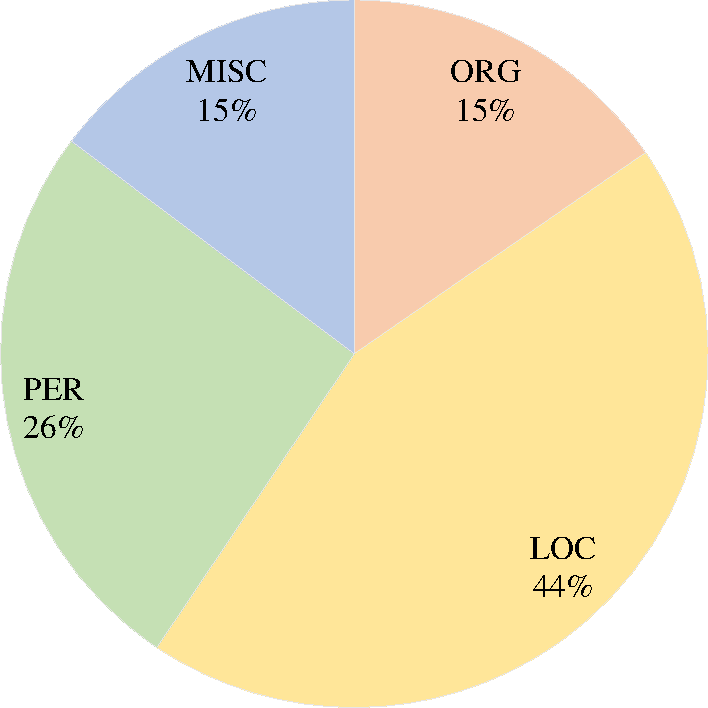
\includegraphics[width=\linewidth]{images/dis-daga.pdf}
    \caption{DAGA}
    \label{fig:daga-conll}
    \end{subfigure}
    \hfill
    \begin{subfigure}[b]{0.45\linewidth}
    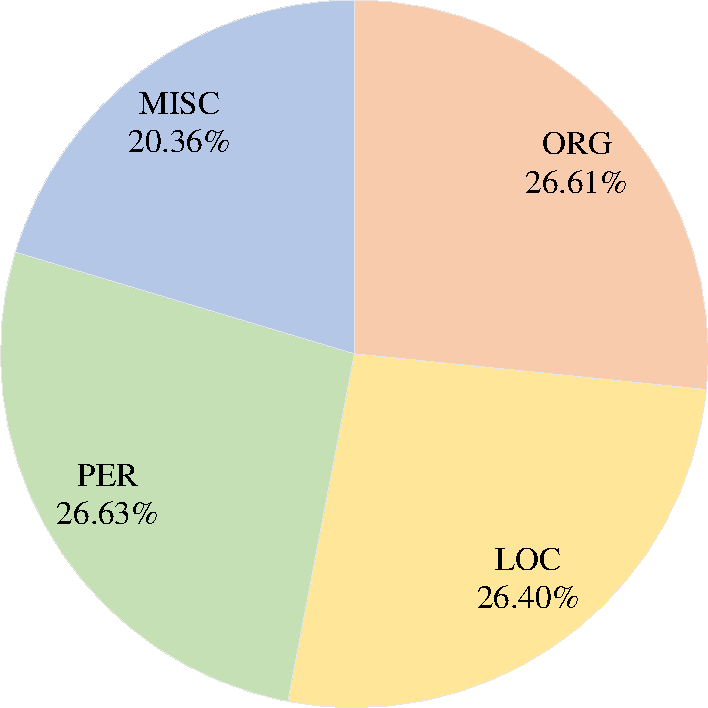
\includegraphics[width=\linewidth]{images/dis-llmda.pdf}
    \caption{LLM-DA}
    \label{fig:ours-conll}
    \end{subfigure}
    \caption{DAGA和LLM-DA (All)增强数据的实体分布。}
    \label{fig:distribution}    
\end{figure}

\subsection{进一步研究}

\paragraph{实体分布}
如第~\ref{sec:intro}节所述，我们旨在使用不同的提示生成数据时在多样性和可控性之间取得平衡。相比之下，DAGA在没有任何限制的情况下生成数据。为比较DAGA和LLM-DA(All)生成的数据，我们在CoNLL'03数据集的20-shot场景下进行比较。图~\ref{fig:distribution}清楚地显示，由于缺乏生成期间的限制，DAGA增强的数据表现出严重不平衡的实体分布。相反，LLM-DA生成的数据具有更均匀的实体分布。通过考虑这一方面，LLM-DA促进了更好的模型训练。

\begin{figure}[!t]
    \centering    
    \begin{subfigure}[b]{0.47\linewidth}
    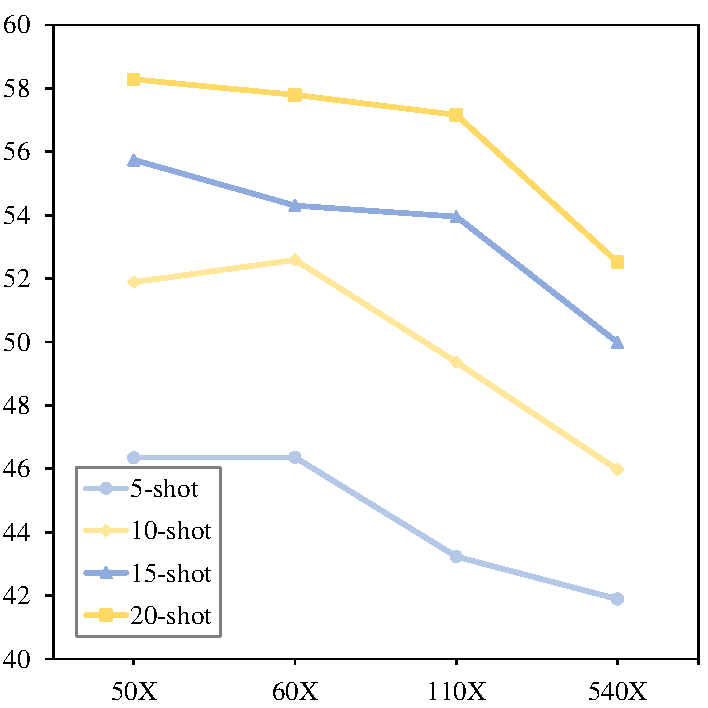
\includegraphics[width=\linewidth]{images/ontonotes.pdf}
    \caption{OntoNotes 5.0}
    \label{fig:onto}
    \end{subfigure}
    \hfill
    \begin{subfigure}[b]{0.47\linewidth}
    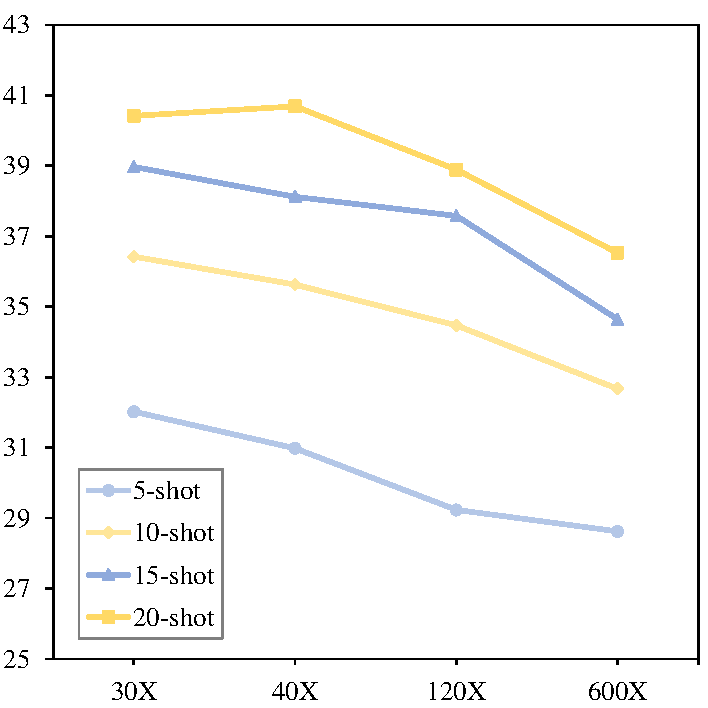
\includegraphics[width=\linewidth]{images/few-nerd.pdf}
    \caption{FEW-NERD}
    \label{fig:few-nerd}
    \end{subfigure}
    \caption{BERT在使用不同增强比的LLM-DA (All)数据时在OntoNotes 5.0和FEW-NERD数据集上的性能。}
    \label{fig:aug-ratio}
\end{figure}

\paragraph{增强数据数量的影响}
为调查模型性能是否随着更高的增强比继续改善，我们以LLM-DA (All)为基础扩展增强比，并在OntoNotes 5.0和FEW-NERD数据集上使用BERT进行实验。如图~\ref{fig:aug-ratio}所示的结果揭示，进一步增加增强比并不能显著提升模型性能；事实上，它甚至导致性能下降。这种现象的出现是因为增强数据是基于预先存在的采样数据生成的，而采样数据本身多样性有限，从而约束了增强数据的质量。随着增强比达到一定阈值，数据多样性达到其上限。继续扩展数据会加剧数据分布与测试数据之间的差异，引入更多噪声从而阻碍模型训练过程。因此，在达到一定量的增强数据后，\emph{更多不一定更好}，提升模型性能的关键在于提高数据质量。

\section{相关工作}

\paragraph{少样本NER任务}
由于NER数据标注的资源密集性，解决少样本NER任务更为实际\cite{fritzler2019few,huang2020few,SNN,template_based,template_free}。虽然当前少样本NER的主要解决方案主要侧重于模型层面的改进，如使用原型网络或基于模板的模型，但我们的工作通过关注数据层面来区分自己。我们的目标是解决少样本场景中NER标注数据不足的根本挑战。

\paragraph{NER任务的数据增强}
NER的数据增强方法可分为句子变换和基于模型生成的方法\cite{LSMS,DAGA,MELM,LAMBADA,DA-intent,Auggpt}。然而，这些方法表现出固有的局限性。它们有可能破坏句子的句法结构或生成与上下文语义不一致的句子，导致模型训练中的过度噪声。在我们的方法中，我们利用LLM为NER生成大量多样化和高质量的新数据。值得注意的是，我们的方法保留了句子的语法和语义结构，确保更有效和准确的训练。

\paragraph{大语言模型}
在大规模文本语料库上训练的LLM在获取庞大世界知识方面展现出卓越的能力。它们已成功应用于某些仅涉及直接重写的简单任务的数据增强。然而，LLM在这些任务中已经表现出高性能，使得进一步的增强变得不必要。我们的方法专门针对NER任务，这凸显了LLM的性能局限性。通过仔细考虑LLM的固有约束和NER的独特特性，我们努力增强LLM在NER任务中的利用。

\section{结论}

本文介绍LLM-DA，一种利用LLM进行少样本NER任务的数据增强方法。我们的方法利用LLM的重写能力和庞大的世界知识，有效解决了现有方法中遇到的句法或语义不一致问题。此外，我们通过在上下文和实体层面纳入提示，在数据多样性和不可预测性之间取得谨慎的平衡。通过大量实验，LLM-DA展现出与当前方法相比的性能优势或同等水平，为提升模型性能做出了宝贵贡献。

\section*{局限性}

尽管我们已努力考虑广泛的场景，但我们的方法也有两个局限性。首先，我们方法中的上下文重写受设计策略的限制，没有使模型适应特定句子领域。尽管如此，我们通过广泛考虑常见领域在一定程度上缓解了这种局限性。其次，LLM有token长度限制，这限制了替换实体的多样性。我们相信，通过扩展实体的生成，可以进一步强调我们方法的优势。

\section*{伦理声明}

我们的方法利用LLM生成独立于现有训练数据的数据，而是从模型在大量预训练数据中获得的知识中汲取。然而，需要注意的是，生成的数据可能继承预训练语料库中存在的社会偏见。因此，我们建议对生成的数据进行人工检查，以减轻在实际应用中将此类偏见传播到下游分类模型的风险。

\bibliography{LLM-DA}

\appendix

\section{LLM-DA的提示词}
\label{appendix:prompts}

我们共设计了17种增强提示词，其中14种用于上下文层面增强（表~\ref{tab:prompts-context}），1种用于实体层面增强（表~\ref{tab:prompts-entity}），1种用于双层增强（表~\ref{tab:prompts-both}），1种用于噪声注入（表~\ref{tab:prompts-noise}）。

\begin{table}[h]
\centering
    \begin{tabular}{m{0.92\linewidth}}
    \toprule
      给定一个句子：""" \\
\{sentence\}\\
"""\\
\\
给定上述句子中以逗号分隔的实体："""\\
\{entities\}\\
"""\\
\\
请使用\{new context\}生成5个新句子。在每个新句子中，每个给定实体只使用一次，保持其在给定句子中的实体类型，不要引入其他实体。\\
\\
期望格式：\\
保留的实体：<所有保留的实体，以逗号分隔>\\
新句子：<新句子>\\
\\
保留的实体：<所有保留的实体，以逗号分隔>\\
新句子：<新句子>
\\ \bottomrule
\end{tabular}
\caption{上下文层面增强的提示词。将"\{sentence\}"替换为原始句子。将"\{entities\}"替换为原始句子中的实体。将"\{new context\}"替换为改写策略。}
\label{tab:prompts-context}
\end{table}

\begin{table}[ht]
\centering
    \begin{tabular}{m{0.92\linewidth}}
    \toprule

给定一个句子："""\\
\{sentence\}\\
"""\\
\\
给定上述句子中以逗号分隔的实体："""\\
\{entities\}\\
"""\\
\\
请生成20个句子，将给定实体替换为同类型的新实体，保持其他词不变。\\
\\
期望格式：\\
替换的实体：<给定实体 -> 新实体, 给定实体 -> 新实体>\\
新句子：<新句子>\\
\\
替换的实体：<给定实体 -> 新实体, 给定实体 -> 新实体>\\
新句子：<新句子>\\ 
\bottomrule
\end{tabular}
\caption{实体层面增强的提示词。将"\{sentence\}"替换为原始句子。将"\{entities\}"替换为原始句子中的实体。}
\label{tab:prompts-entity}
\end{table}

\begin{table}[ht]
\centering
    \begin{tabular}{m{0.92\linewidth}}
    \toprule
给定一个句子："""\\
\{sentence\}\\
"""\\
\\
给定上述句子中以逗号分隔的实体："""\\
\{entities\}\\
"""\\
\\
请将给定实体替换为同类型的新实体，保持其他词不变。\\
\\
期望格式：\\
替换的实体：<给定实体 -> 新实体, 给定实体 -> 新实体>\\
新句子：<新句子>\\ \bottomrule
\end{tabular}
\caption{双层增强的提示词。将"\{sentence\}"替换为原始句子。将"\{entities\}"替换为原始句子中的实体。}
\label{tab:prompts-both}
\end{table}

\begin{table}[ht]
\centering
    \begin{tabular}{m{0.92\linewidth}}
    \toprule
 给定一个句子："""\\
\{sentence\}\\
"""\\
\\
给定上述句子中以逗号分隔的实体："""\\
\{entities\}\\
"""\\
\\
请在给定句子中随机使用一些常见拼写错误。\\
\\
期望格式：\\
替换的实体：<给定实体 -> 新实体, 给定实体 -> 新实体>\\
新句子：<新句子>\\
\bottomrule
\end{tabular}
\caption{噪声注入的提示词。将"\{sentence\}"替换为原始句子。将"\{entities\}"替换为原始句子中的实体。}
\label{tab:prompts-noise}
\end{table}

\section{处理NER任务的提示词}
\label{appendix:gpt}

为了评估ChatGPT在NER任务上的性能，我们设计了特定的提示词，直接使用gpt-3.5-turbo处理这些任务，如表~\ref{tab:prompts-gpt}所示。

\begin{table}[ht]
    \centering
    \begin{tabular}{m{0.17\linewidth}|m{0.7\linewidth}}
    \toprule
    \# Shot & \multicolumn{1}{c}{提示词} \\ \midrule
    \multirow{6}*{零样本} & 请从给定文本中识别\{entity\_categories\}实体。\\
    ~ & ~\\
    ~ & 期望格式：\{format\}\\
    ~ & ~\\
    ~ & 文本：\{sentence\}\\
    ~ & 实体：\\ \midrule

    \multirow{6}*{少样本} & 请从给定文本中识别\{entity\_categories\}实体。\\
    ~ & ~\\
    ~ & \{examples\}\\
    ~ & ~\\
    ~ & 文本：\{sentence\}\\
    ~ & 实体：\\
    \bottomrule
    \end{tabular}
    \caption{为gpt-3.5-turbo直接执行NER任务设计的提示词。将"\{entity\_categories\}"替换为数据集中的实体类别。将"\{sentence\}"替换为待识别的句子。将"\{format\}"替换为零样本设置中的期望输出格式。将"\{examples\}"替换为少样本设置中的示例。}
    \label{tab:prompts-gpt}
\end{table}

\end{document}
